Neste capítulo mostraremos exemplos de resultados de utilização da ferramenta, para isso demonstraremos com alguns códigos simples a interação com o sistema e seus resultados, como também alguns exemplos de erros de montagem que são tratados neste projeto.

Para vermos melhores resultados, criamos os seguintes códigos,

\begin{itemize}
	\item Aritmética simples
	\item Sequência de Fibonacci
	\item Preenchimento Bitmap 
\end{itemize}


\section{Possíveis erros de montagem}

	Como explicado na seção anterior, sendo a montagem, a parte que lida diretamente com a entrada do usuário, é necessário que o sistema saiba lidar com possíveis erros inseridos no código e devolver uma resposta adequada. Foram implementados as seguintes mensagens de erro:
	
	 Na figura \ref{fig:assemble_error_duplicated_symbol}, temos um exemplo de erro de declaração múltipla de símbolo, ou seja, se o programador declarar o mesmo símbolo em dois momentos diferentes no código.
	
	\begin{figure}[h!]
	  \centering
	  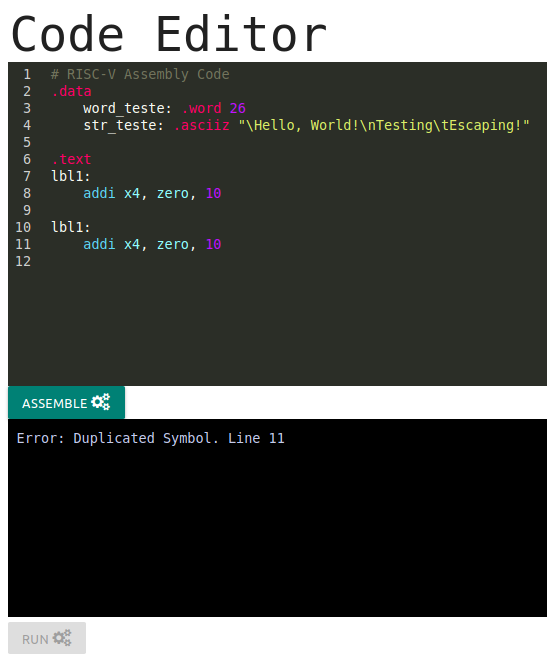
\includegraphics[width=8cm]{img/assemble_error_duplicated_symbol.png}
	  \caption{Erro de declaração múltipla de símbolo.}
	  \label{fig:assemble_error_duplicated_symbol}
	\end{figure}

	 Na figura \ref{fig:assemble_error_directives_strings}, temos um exemplo de erro da diretiva .asciiz ou .string, quando é declarado mais de uma string para um único símbolo.
	

	\begin{figure}[h!]
	  \centering	  
	  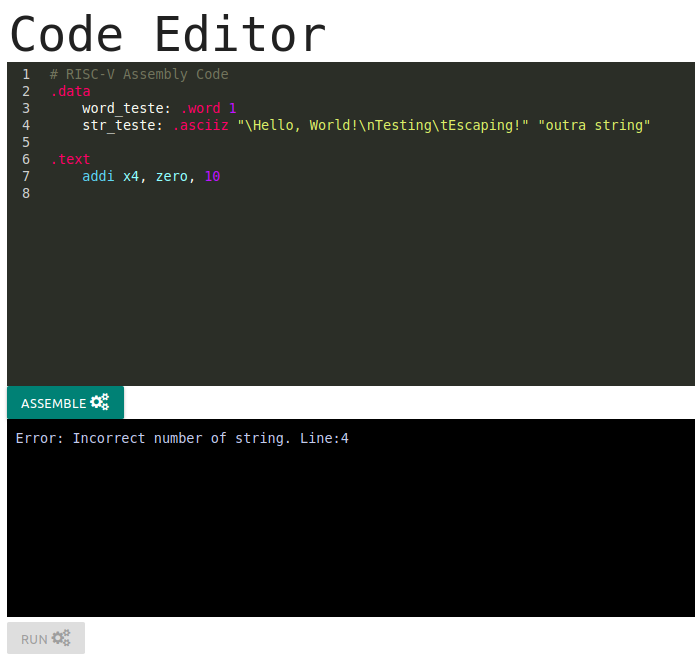
\includegraphics[width=8cm]{img/assemble_error_directives_strings.png}
	  \caption{Erro de declaração de diretiva string.}
	  \label{fig:assemble_error_directives_strings}
	\end{figure}


	 Na figura \ref{fig:assemble_error_imediato}, temos um exemplo de erro de valor de imediato, no caso deste projeto onde utilizamos tamanhos de palavra 12 bits, um valor superior a 2047 ou inferior a -2047 traria um overflow.
	
	\begin{figure}[h!]
	  \centering
	  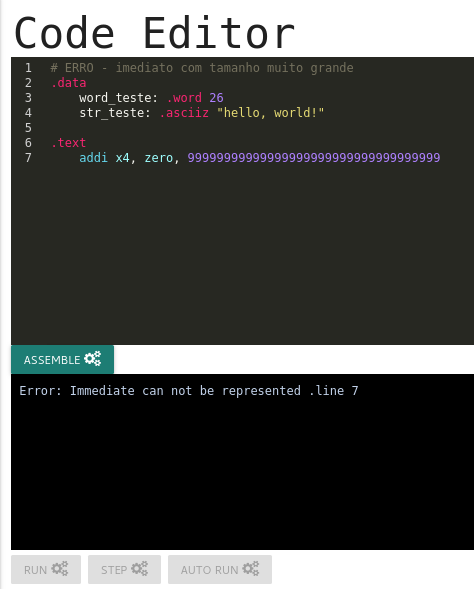
\includegraphics[width=8cm]{img/assemble_error_imediato.png}
	  \caption{Erro de imediato para o tamanho de palavra 12 bits.}
	  \label{fig:assemble_error_imediato}
	\end{figure}
	 Na figura \ref{fig:assemble_error_operando_invalido}, temos um exemplo de erro de operando inválido, a instrução ADDI pede um imediato como último argumento, porém é fornecido um registrador.
	
	\begin{figure}[h!]
	  \centering
	  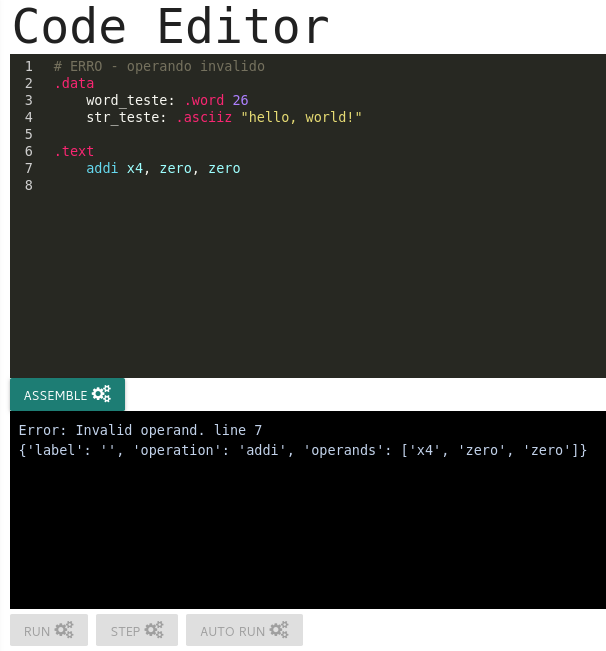
\includegraphics[width=8cm]{img/assemble_error_operando_invalido.png}
	  \caption{Erro de operando inválido, operando de tipo diferente do esperado.}
	  \label{fig:assemble_error_operando_invalido}
	\end{figure}

	 Nas figuras \ref{fig:assemble_error_operation_not_recognized}, e \ref{fig:assemble_error_op_not_recog_directives}, temos um exemplo de erro de operação não reconhecida, sendo que o primeiro mostra que foi fornecido uma instrução desconhecida, e no segundo uma diretiva desconhecida.

	\begin{figure}[h!]
	  \centering
	  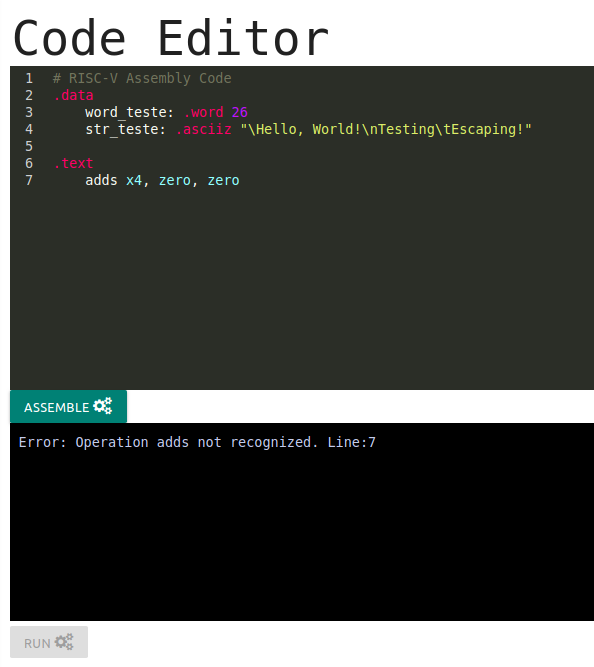
\includegraphics[width=8cm]{img/assemble_error_operation_not_recognized.png}
	  \caption{Erro de operação inválida, instrução não existente na arquitetura implementada.}
	  \label{fig:assemble_error_operation_not_recognized}
	\end{figure}

	\begin{figure}[h!]
	  \centering
	  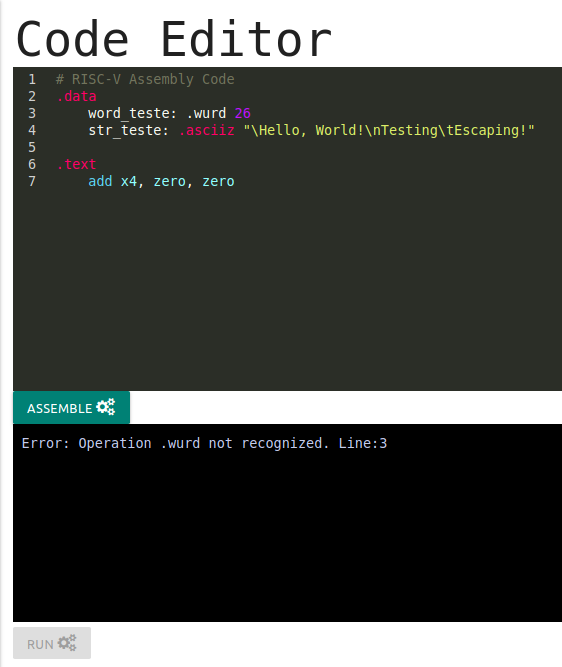
\includegraphics[width=8cm]{img/assemble_error_op_not_recog_directives.png}
	  \caption{Erro de operação inválida, diretiva não existente na arquitetura implementada.}
	  \label{fig:assemble_error_op_not_recog_directives}
	\end{figure}

	 Na figura \ref{fig:assemble_error_simbolo_inexistente}, temos um exemplo de erro de símbolo inexistente, o programador tentou utilizar um símbolo que não foi declarado antes.
	\begin{figure}[!]
	  \centering
	  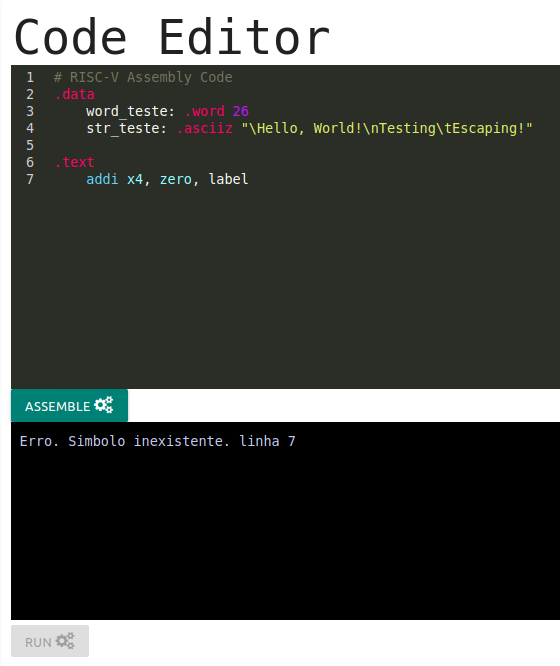
\includegraphics[width=8cm]{img/assemble_error_simbolo_inexistente.png}
	  \caption{Erro de símbolo inválido, símbolo não foi declarado.}
	  \label{fig:assemble_error_simbolo_inexistente}
	\end{figure}

	 Na figura \ref{fig:assemble_error_wrong_arguments}, temos um exemplo de erro de tipo ou número de argumentos de diretiva, parecido com o erro da figura \ref{fig:assemble_error_directives_strings}. Neste exemplo a diretiva .word pede um número e lhe é fornecido outra label.

	\begin{figure}[h!]
	  \centering
	  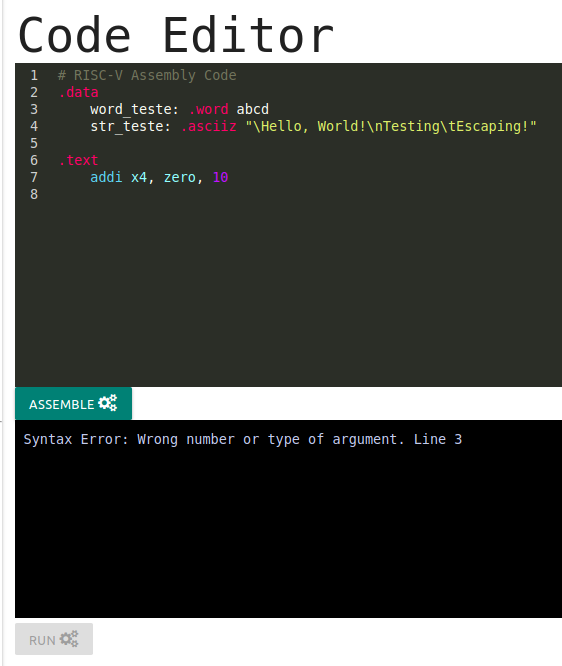
\includegraphics[width=8cm]{img/assemble_error_wrong_arguments.png}
	  \caption{Erro de argumentos de diretiva inválido, o tipo ou número de argumentos está incorreto.}
	  \label{fig:assemble_error_wrong_arguments}
	\end{figure}




\section{Aritmética Simples}
	
	Este código mostra algumas instruções matemáticas básicas, de registrador para registrador, muito utilizadas em uma variedade de programas. Neste código poderemos ver a utilização destas instruções e seus resultados em cada registrador separado, verificando suas funcionalidades.

\subsection{Editor de código}


	Na figura \ref{fig:operacoes_matematicas_codigo} está o código que utilizamos para demonstração de algumas das instruções matemáticas mais básicas. Neste exemplo foi utilziada a instrução ADDI para inicializar valores nos registradores x3 e x4. A partir dos valores contidos nestes registradores realizamos várias operações matemáticas, ADD (adição), SUB (subtração), SRL (shift right logical), SLL (shift left logical), AND, OR, XOR, SLT (set less than). 

	\begin{figure}[h]
	  \centering
	  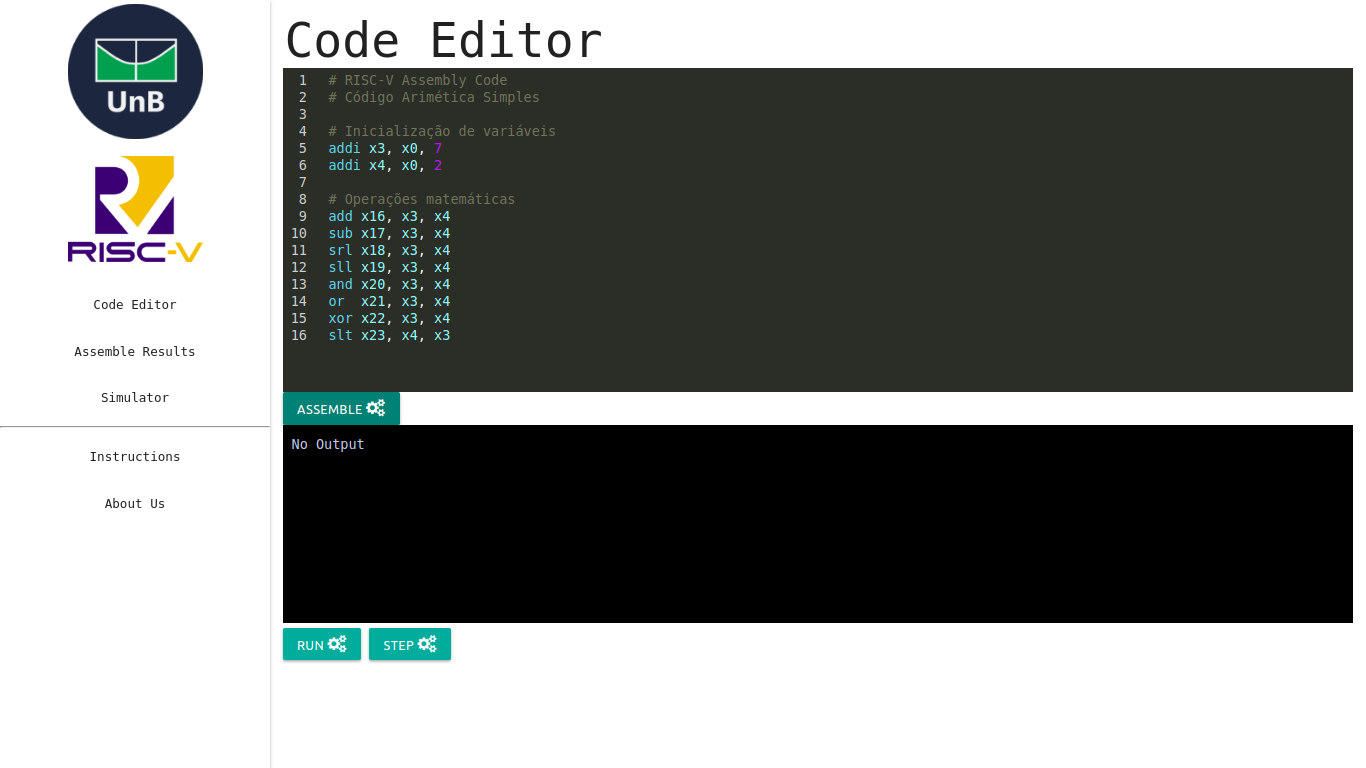
\includegraphics[width=8cm]{img/aritmetica_codigo.png}
	  \caption{Demonstração de operações matemáticas básicas.}
	  \label{fig:operacoes_matematicas_codigo}
	\end{figure}


\subsection{Simulação}
	
	Para cada operação realizada com estes valores, cada resultado foi armazenado em um registrador do x16 ao x23, como podemos ver na figura \ref{fig:operacoes_matematicas_resultados}

	\begin{figure}[h]
	  \centering
	  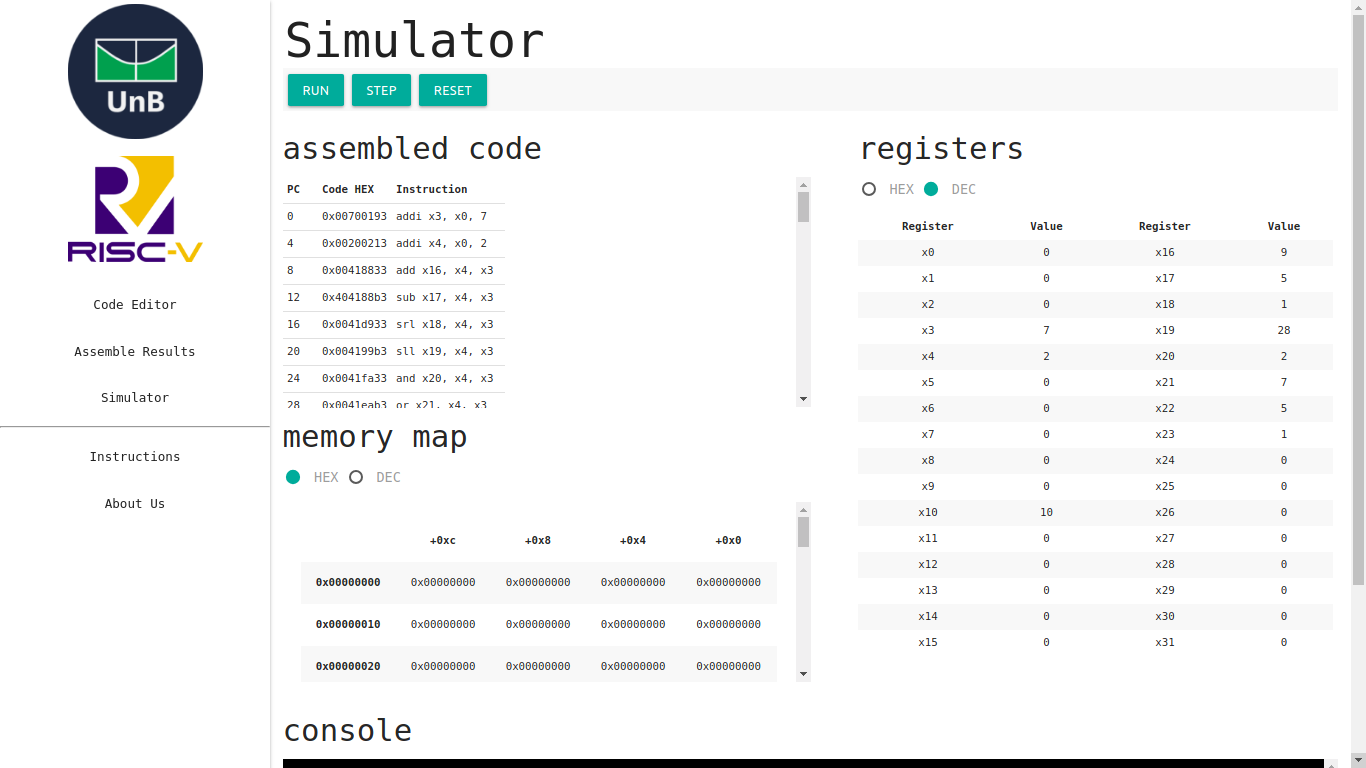
\includegraphics[width=8cm]{img/aritmetica_results.png}
	  \caption{Demonstração de operações matemáticas básicas.}
	  \label{fig:operacoes_matematicas_resultados}
	\end{figure}

	Como o programa não escreve na memória ou imprime resultados na tela, os resultados importantes a serem ressaltados são os valores de registradores e também o código montado. Os valores dos registradores são mostrados na forma decimal.


\section{Sequência de Fibonacci}
	
	A sequência de fibonacci é um dos primeiros algoritmos que aprendemos quando iniciamos nos estudos de programação. Cada termo desta sucessão de números é gerada pela soma dos dois números antecedentes.

\subsection{Editor de código}


	Na implementação do algoritmo de Fibonacci abaixo temos a inicialização de duas variáveis, n\textunderscore fibs, que é a quantidade de termos da sequência que desejamos obter. A outra variável é a fib\textunderscore base\textunderscore mem\textunderscore addr. O valor atribuído a esta variável não é relevante neste programa, apenas denota a base de endereço onde serão armazenados os termos.

	Depois temos a função fib, que inicializa registradores. Colocando em x3 como o número de termos que serão escritos. Em x4 o primeiro termo de fibonacci, em x6 um valor auxiliar, em x10 atribuímos o valor 1 para chamadas de impressão de inteiros através de \textit{ecalls}. Ainda podemos ver uma parte da função loop, que irá calcular novos termos. A primeira instrução BEQ serve para verificarmos se já atingimos o número de termos desejados. Após a verificação faz-se um salto para funções de impressão. Vemos também a utilização do registrador x7, que servirá de auxiliar para não perdemos o valor de atual do termo de fibonacci. Então o registrador x4 recebendo a soma do próprio x4 que é o valor atual do termo de fibonacci e x6 que é o valor auxiliar.

	\begin{verbatim}
        # RISC-V Assembly Code
        # Fibonacci
        .data
            n_fibs: .word 8
            fib_base_mem_addr: .word 16
        .text
        fib:
            lw x3, n_fibs(x0) # counter
            addi x4, x0, 1  # fib number
            addi x6, x0, 0 # fib aux

            addi x10,zero,1
        loop:
            beq x3, x0, end

            jal x20, print_to_console
            jal x21, print_to_mem

            addi x7, x4, 0 #aux = fib
            add x4, x4, x6  # fib = fib+fib_aux
            addi x6,x7,0 # fib_aux = aux
		    
            addi x3,x3, -1 #dec counter
            jal x0, loop

        print_to_console:
            addi x5,x4,0  
            ecall# print value
            jalr x0, x20, 0

        print_to_mem:
            sw x4, fib_base_mem_addr(x30)
            addi x30, x30, 4
            jalr x0, x21, 0

        end: 


	\end{verbatim}


	Na continuação da função loop, mostrado no código acima, somamos o valor em x7, valor do termo anterior, com 0 e adicionamos em x6, variável auxiliar de fibonacci.

	Após encontrar os termos terem sido atualizados para o próximo laço se faz um decremento do valor do registrador x3, que contém a quantidade de termos que o usuário deseja, que foi obtido a partir da label n\textunderscore fibs.

	Depois de decrementado o valor, se faz um salto para o início do loop, onde vai ser verificado se já foram encontrados todos os valores desejados e se pode pular para a \textit{label end} e encerrar o programa. 

	Em seguida, nas linhas 25 e 30, estão as labels para as chamadas das rotinas de impressão chamadas dentro da função \textit{loop}, \textit{print\textunderscore to\textunderscore console}, e \textit{print\textunderscore to\textunderscore mem}. Estas rotinas não utilizam a pilha para variáveis e retornos, como se utilizassem apenas variáveis globais.

	A função \textit{print\textunderscore to\textunderscore console} simplesmente move o valor de x4, termo de fibonacci, para o registrador x5, que é utilizado dentro da instrução ECALL (\textit{environment call}). E então retornamos ao loop com a instrução JALR.

	A outra função, \textit{print\textunderscore to\textunderscore mem}, faz um SW (\textit{store word}) do valor contido no registrador x4 no endereço dado pela soma do valor de x30 adicionado do endereço da variável de fib\textunderscore base\textunderscore mem\textunderscore addr. Depois adicionamos 4 em x30 para que no próximo laço seja impresso o próximo inteiro no endereço de \textit{store word} correto. E então retornamos ao \textit{loop}.

	Ao final do código devemos ter o número de termos de fibonacci fornecidos pelo usuário mostrado tanto na console de saída quanto em endereços na memória.


\subsection{Simulação}

	
	Na primeira parte dos resultados demonstrados na figura \ref{fig:fib-results-1} vemos parcialmente o código montado gerado pelo montador, valores residuais dos registradores utilizados e os valores da memória.

	\begin{figure}[h]
	  \centering
	  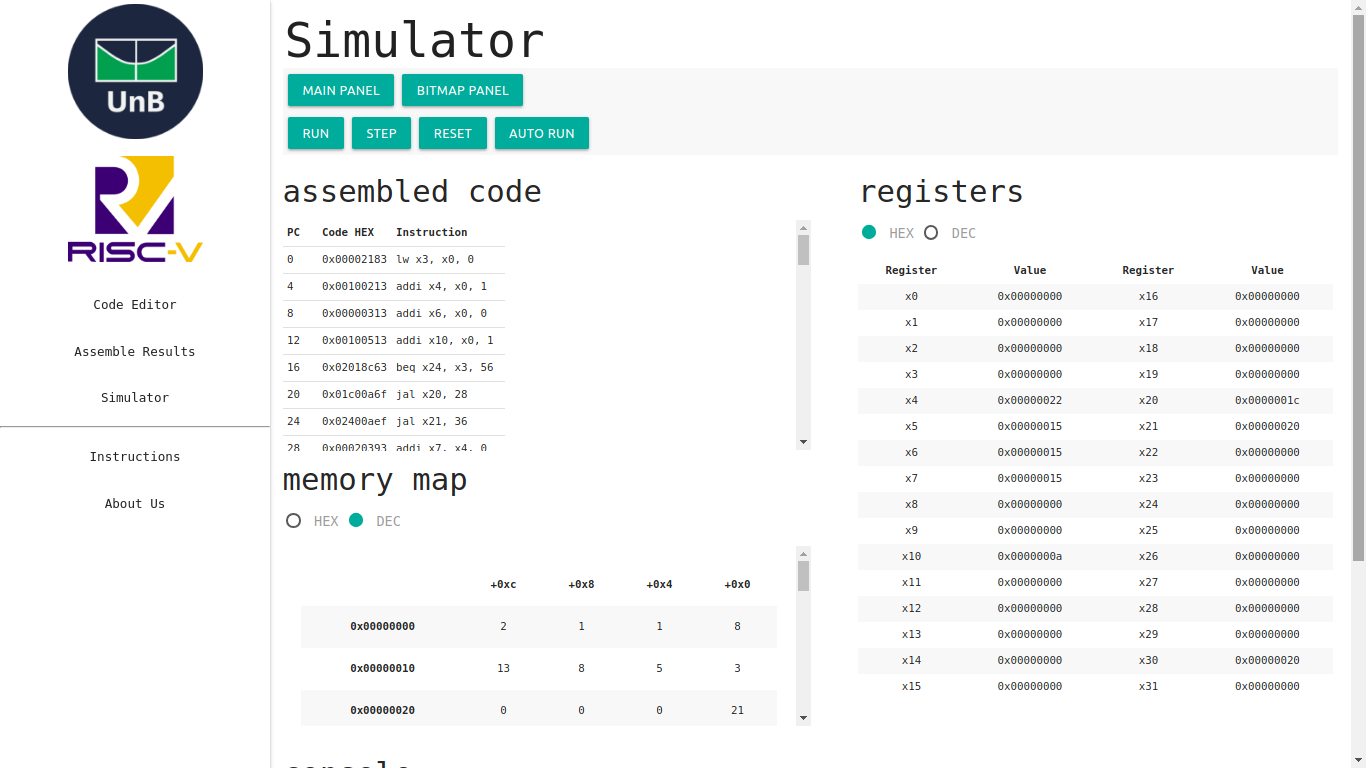
\includegraphics[width=14cm]{img/fibonacci_results_1.png}
	  \caption{Primeira parte dos resultados gerados da sequência de fibonacci.}
	  \label{fig:fib-results-1}
	\end{figure}

	Na primeira instrução vemos que o programa executa um Load Word no endereço 0 da memória, este endereço contém o valor fornecido pelo programador com o número de termos de fibonacci que gostaria de obter. A partir do segundo endereço, o 0x00000004, temos a sequência de valores de fibonacci impressos na memória a cada iteração do loop.

	Na figura \ref{fig:fib-results-2} podemos ver a console de saída. Esta parte nos mostra a funcionalidade da chamada de ambiente, ou ECALL, que imprime um número inteiro na tela. 

	\begin{figure}[h]
	  \centering
	  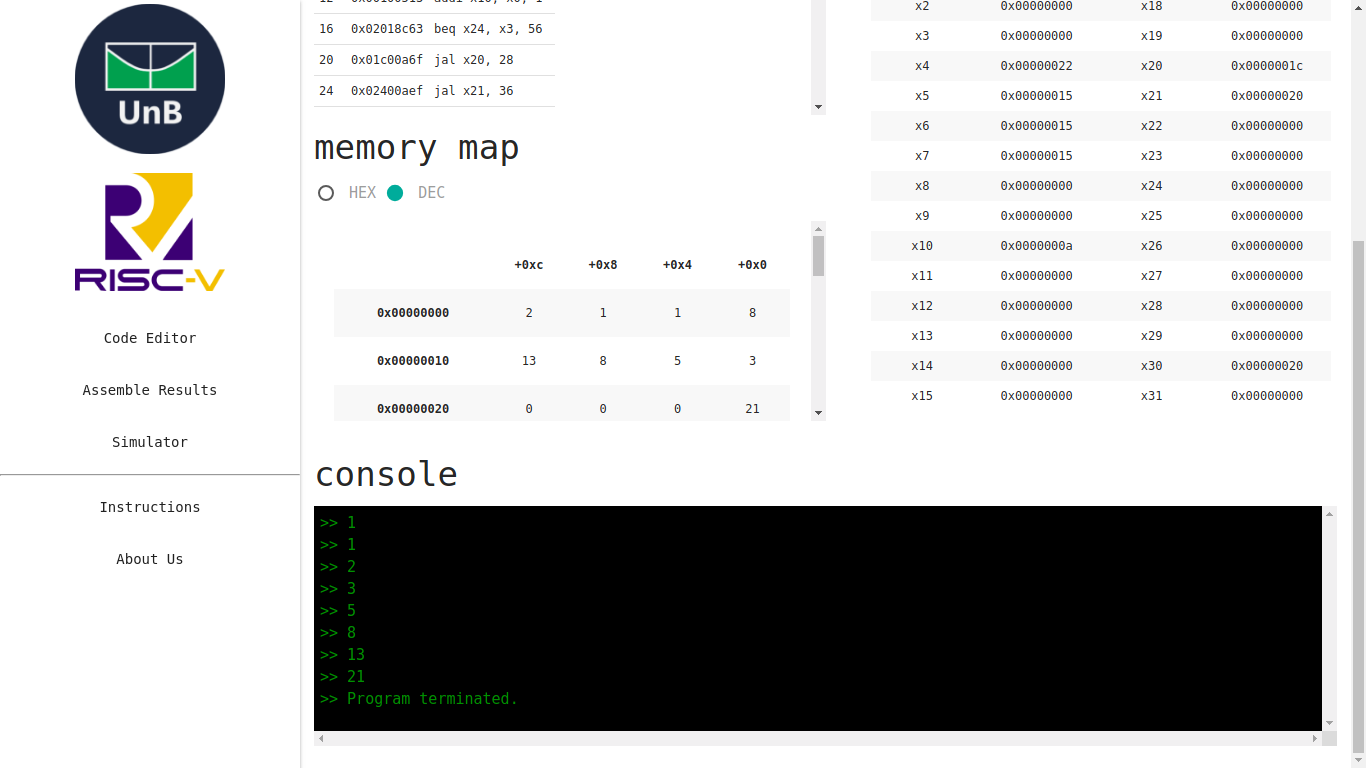
\includegraphics[width=14cm]{img/fibonacci_results_2.png}
	  \caption{Segunda parte dos resultados gerados da sequência de fibonacci.}
	  \label{fig:fib-results-2}
	\end{figure}

	Os termos foram impressos um em cada linha, cada linha representa uma chamada da instrução ECALL com o valor 1 no registrador x10, e o termo a ser impresso contido no registrador x5. Ao final do código temos a outra chamada de ambiente implementada que é a de saída do programa, chamando ECALL com o valor 10 no registrador x10.


\section{Preenchimento Bitmap}

	Este código simplesmente adiciona o valor 255(0x0000ff) nas áreas de memória de endereço 256(0x100) até o endereço 1276(0x4fc) para visualizarmos melhor e criar programas como o jogo da vida de John Conway~\cite{conway1970game}.

\subsection{Editor de código}

	No código da figura \ref{fig:codigo-bitmap}, temos três variáveis inseridas previamente, com o valor em decimal da cor azul, o endereço inicial da região de memória que é representada pelo painel, e a quantidade de endereços que serão inseridos. No bloco main apenas é buscado os valores da memória para registradores.
	
	\begin{figure}[h!]
	  \centering
	  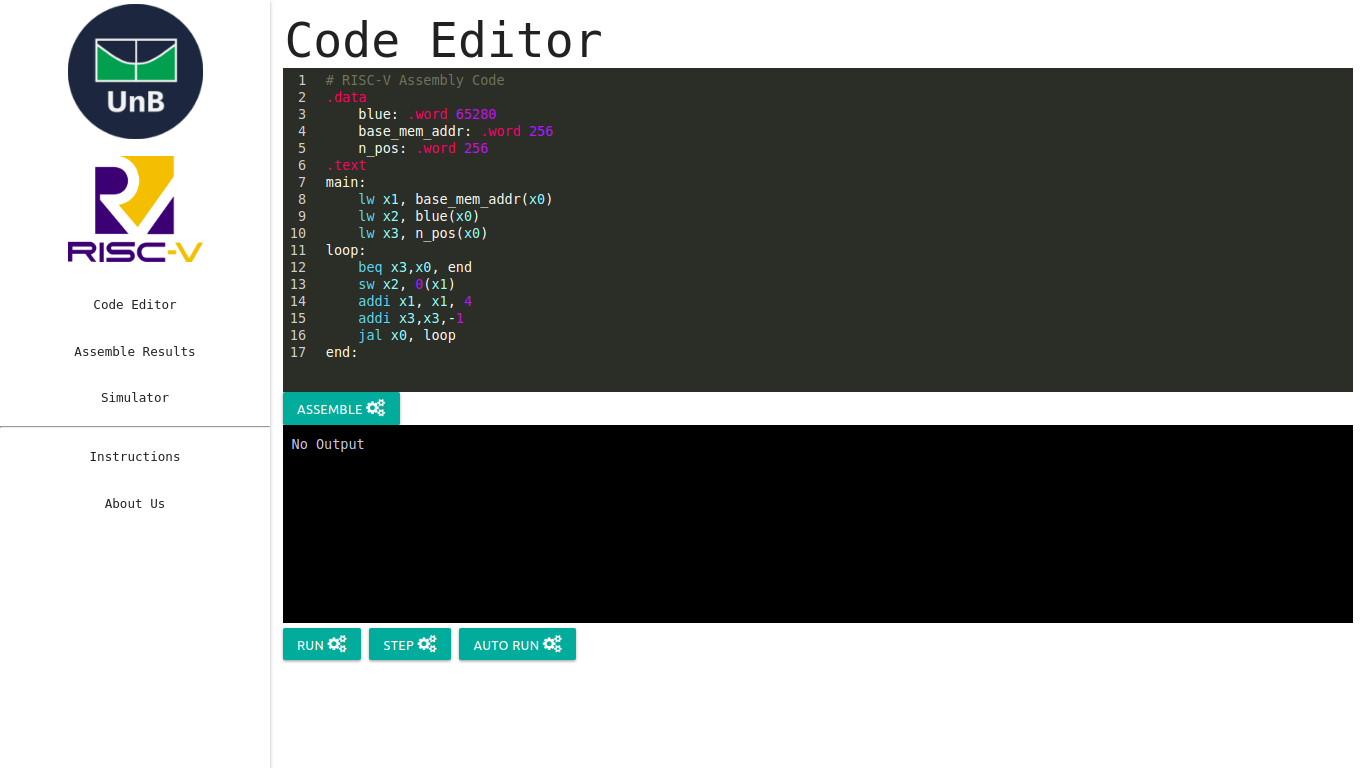
\includegraphics[width=14cm]{img/codigo_bitmap.png}
	  \caption{Código de exemplo de utilização do painel de Bitmap para representação de região da memória.}
	  \label{fig:codigo-bitmap}
	\end{figure}

	Em seguida, ao entrar no loop, testa se o valor de n\textunderscore pos que foi inserido em x3 é zero, se for pula para a label end e que encerra o programa. Caso o valor de x3 não seja zero continua a execução do loop. Na continuação do loop se insere o valor de blue no endereço base\textunderscore mem\textunderscore addr, depois adiciona-se 4 para na próxima iteração pegar o endereço relativo à próxima word. Por fim decrementa-se o valor do contador e volta ao início do loop.


\subsection{Simulação}
	
	Na figura \ref{fig:simulation-bitmap-bitmap-panel}, vemos o painel Bitmap e a execução está acontecendo no modo AUTO RUN, para que possamos ver a dinâmica do programa. Neste painel, não podemos ver os registradores e a console de saída, porém ao clicar no botão MAIN PANEL pode-se ver esses valores atualizados.

	\begin{figure}[h!]
	  \centering
	  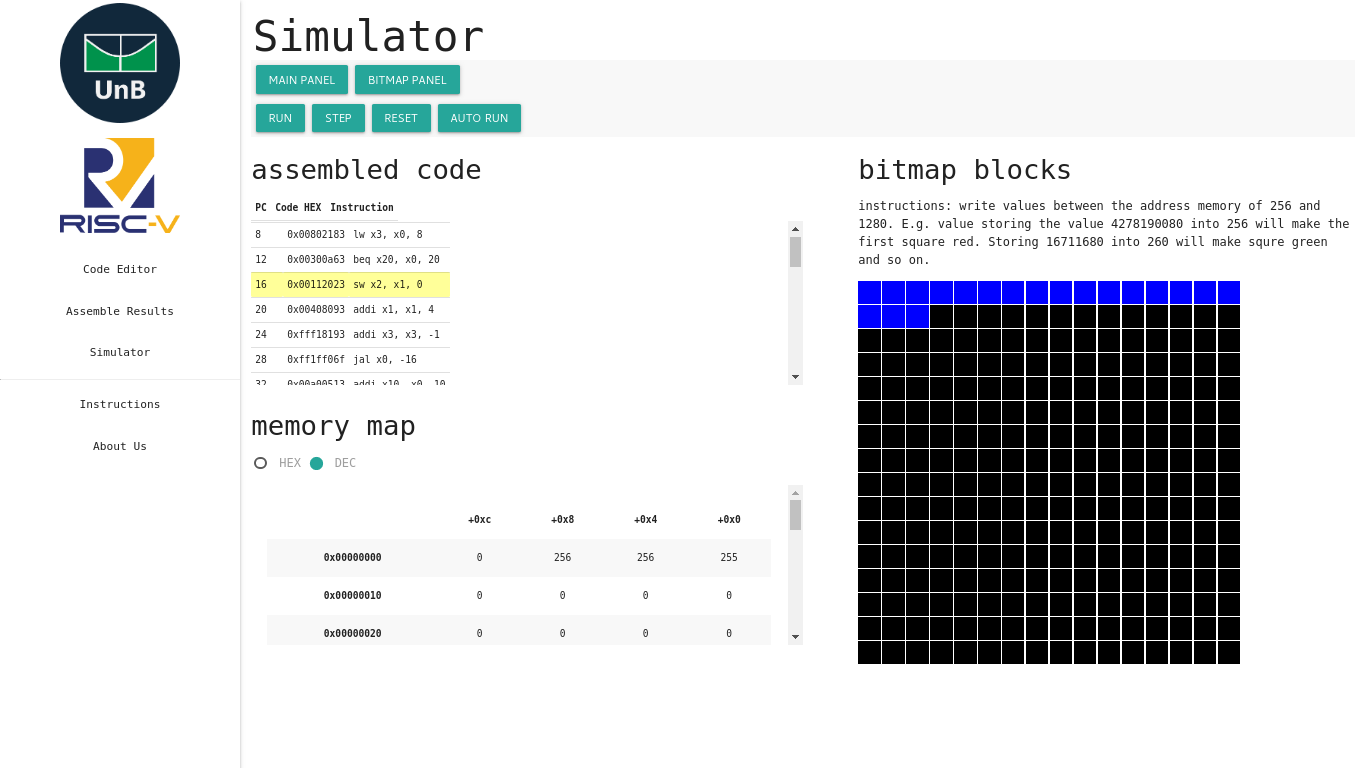
\includegraphics[width=14cm]{img/simulation_bitmap_bitmap_panel.png}
	  \caption{Resultado parcial do código de exemplo de utilização do painel de Bitmap para representação de região da memória.}
	  \label{fig:simulation-bitmap-bitmap-panel}
	\end{figure}

	Na figura \ref{fig:simulation-bitmap-main-panel}, podemos ver o valores dos registradores, sendo que o x1 contém o valor do endereço que será colorido, e no x3 quantos blocos faltam ser coloridos para terminar o preenchimento.

	\begin{figure}[h!]
	  \centering
	  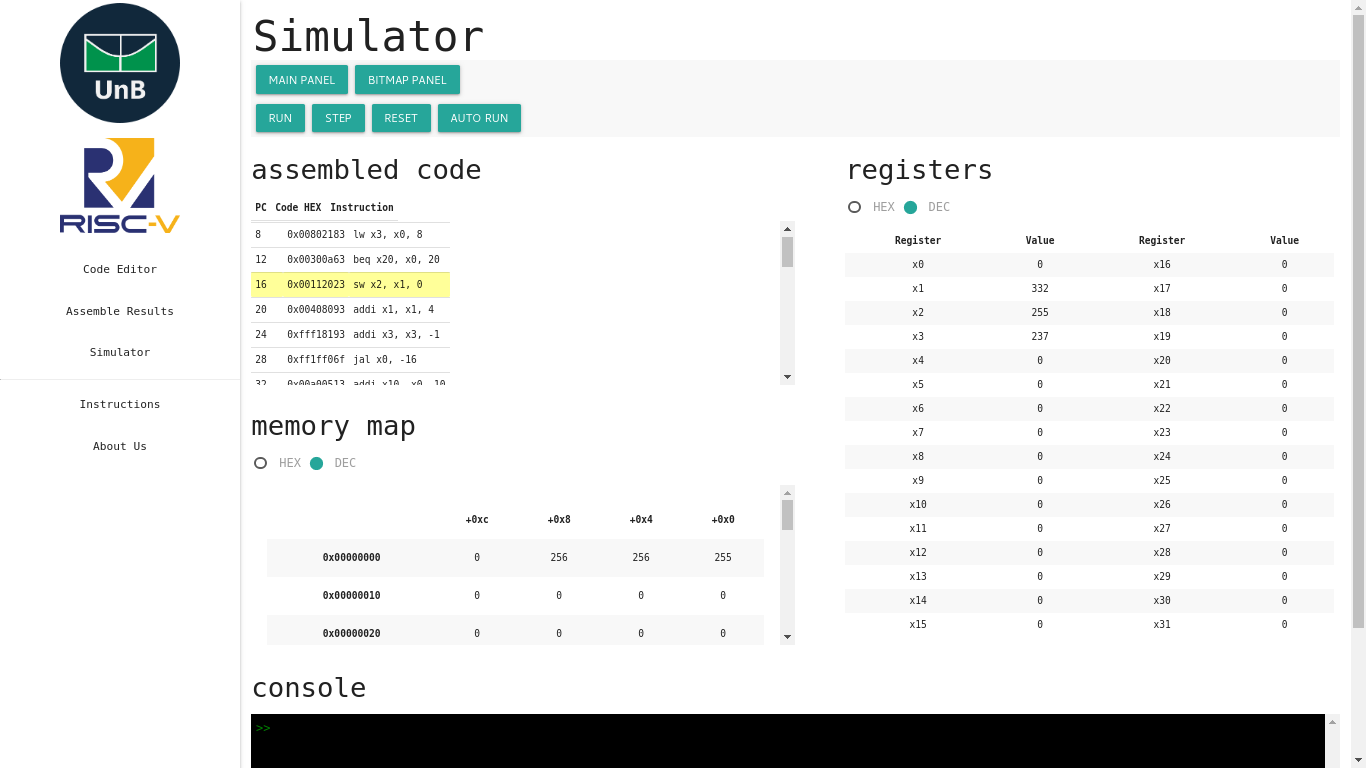
\includegraphics[width=14cm]{img/simulation_bitmap_main_panel.png}
	  \caption{Resultado parcial do código de exemplo de utilização do painel principal que mostra os registradores e console de saída.}
	  \label{fig:simulation-bitmap-main-panel}
	\end{figure}

	Podemos ver também no mapa de memória os endereços que estão em azul com o valor 255 e os que estão em preto com o valor 0.